\documentclass[aspectratio=169]{beamer}              % only frames

% for themes, etc.
\mode<presentation>
\usetheme{Madrid} 
\usecolortheme{crane}

%\usepackage{times}  % fonts are up to you
% The usual suspects
\usepackage{multirow, booktabs, dcolumn, color, graphicx} % Tables\usepackage{graphicx}
\usepackage{amsmath,amssymb,amsthm}
% Strikethrough text
\usepackage{soul}
% Adjust box to fit tabulars
\usepackage{adjustbox}
% Embed video
\usepackage{media9}
% For notes
\usepackage{pgfpages}
%\setbeameroption{hide notes} % Only slides
%\setbeameroption{show only notes} % Only notes
\setbeameroption{show notes on second screen=right} % Both
% Give a slight yellow tint to the notes page
%\setbeamertemplate{note page}{\pagecolor{yellow!5}\insertnote}\usepackage{palatino}
% Use colors by name
\usepackage{xcolor}
% EMBEDDING VIDEO IS POSSIBLE WITH PDFPC USE PDF PC to present
\usepackage{multimedia}



% The table highlighting for hypothesis discussion.
\usepackage[beamer,customcolors]{hf-tikz}
\usetikzlibrary{calc}

% To use background images
\newenvironment{colorframe}[2][]{%
\setbeamercolor{background canvas}{bg=#1}
\begin{frame}\color{white}}
{\end{frame}}


% To set the hypothesis highlighting boxes red.
\tikzset{hl/.style={
    set fill color=red!80!black!40,
    set border color=red!80!black,
  },
}

% Set Graphics folder
\graphicspath{{./figures/}}


% these will be used later in the title page
\title{Scams, Cons, Propaganda and Social Engineering}
\author{Irfan Kanat}
\institute[CBS]{{Department of Digitization}\\ Copenhagen Business School}
\date{\today}



\begin{document}

% this prints title, author etc. info from above
\begin{frame}

	\titlepage

    \vfill
    {\tiny This work is licensed under a \href{http://creativecommons.org/licenses/by/4.0/}{Creative Commons Attribution 4.0 International License}.}

\end{frame}

\note{In this module we will talk about how our psychology makes us vulnerable to manipulation and what we can do to resist it.}

\begin{frame}
    \frametitle{Social Engineering}

    \centering

    \movie{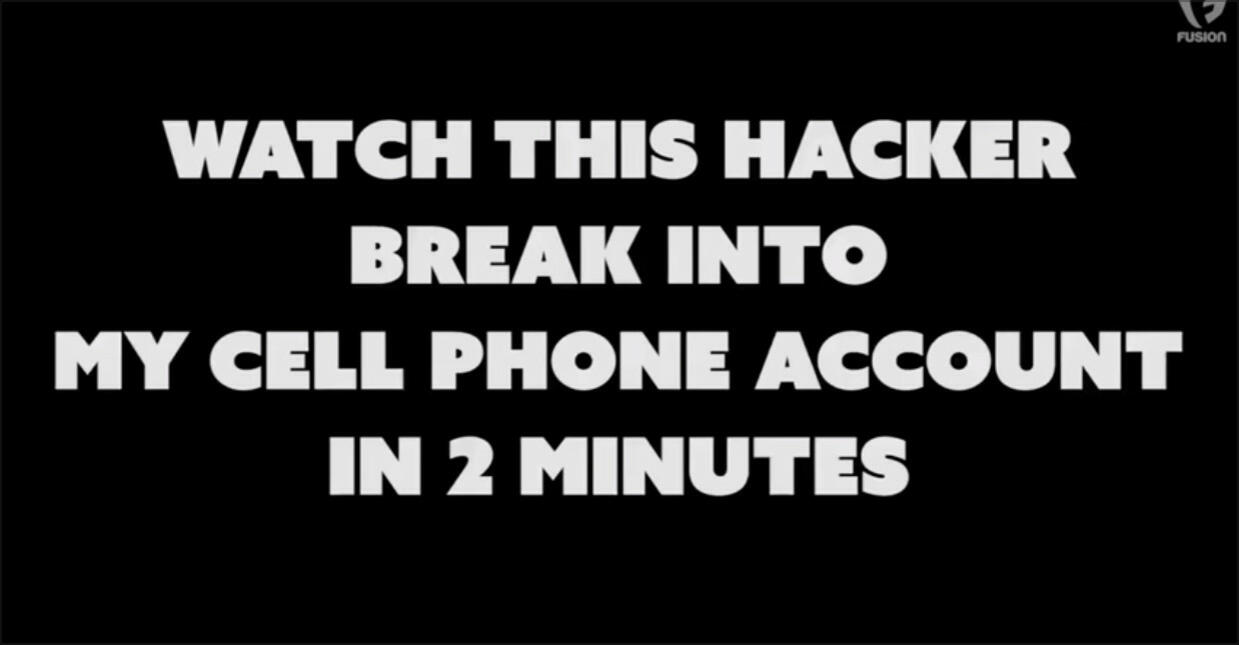
\includegraphics[width = \textwidth]{figures/SocEng.jpg}}{figures/SocEng.mp4}   

\end{frame}

\note{}

\begin{frame}
    \frametitle{Notice What She Did}
    
        \begin{columns}
            \begin{column}{0.5\textwidth}

                \begin{itemize}
                    \item Urgency
                    \item Empathy
                \end{itemize}
        
            \end{column}
    
            \begin{column}{0.5\textwidth}
    
                
\includegraphics[width = \textwidth, height = .85\textheight, keepaspectratio]{figures/CryBaby.png}
    
            \end{column}
    
        \end{columns}

\end{frame}

\note{She created a sense of urgency. ``My husband told me to get it done today.'', ``I can't call you back.''

Then she created a situation where the otherside would want to help her. Who is heartless enough to say ``NO'' to a mother with a crying baby?}


\begin{frame}
    \frametitle{There is More}
    
    \begin{itemize}
        \item Authority
        \item Fear
        \item Hope
        \item In-group/Out-group
        \item \ldots
    \end{itemize}

\end{frame}

\note{
    It is weird but when I came to Denmark, I kept getting calls from ``Microsoft'' about a virus in my operating system which they needed to urgently fix. Hackers were about to do untold horrific things to me if I did not immediately comply with them. It is funny, because I have no Windows computers except for a few virtual machines I turn on when I need to make tutorials.

    There are many examples: In US: IRS calling about tax fraud (IRS doesn't call, they send a letter). In Turkey: Police calling about Terrorists receiving financial support from your bank account \ldots

    What is common in all of them is that the adversary will use emotions that will make you suspend your logic and take ill advised actions.
}

\begin{frame}
    \frametitle{Not Just on The Phone}
    
    \centering

    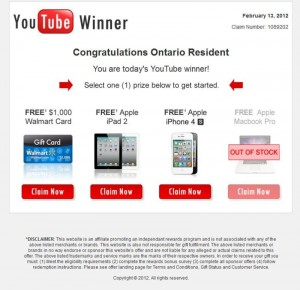
\includegraphics[width = \textwidth, height = .85\textheight, keepaspectratio]{figures/OldTrick.jpg}

\end{frame}

\note{Any medium can be used for manipulation.

Here, notice the claim number on the top right. It lends an air of legitimacy.

Geo-location based on network addresses to make it look more real. Mixing some truth with a lie makes the lie go down easier.

It urges the person to select one gift. So it engenders feelings of hope. You would want a gift. Your brain is already reaching out to accept it. 

BUT if you have any doubts, there is a Macbook pro that is out of stock. If you don't act now, the rest of it can also run out... There is urgency.}

\begin{frame}
    \frametitle{Phishing: Social Engineering in Your In-Box}

    \begin{quote}
        Give a man an exploit and he will have access for a day, teach phishing and he will have access all his life.
    \end{quote}
    \vspace{1em}
    \hfill Phineas Phisher, Hacktivist, 2019 \hspace{2em}
    
\end{frame}

\note{By some estimates phishing is how 90\% of all breaches start. I can't vouch for that figure, bit I think it is important that you know what it is.

Some consider phishing to be a form of social engineering. 

This is the practice of sending e-mails with malicious attachments, links.

In its crudest form, you would play the margins. You would send a generic e-mail to thousands of people (employees) in the hopes some percentage will click on it.

It can also get pretty specific, an e-mail designed to attract one particular person with an e-mail that appears to come from your family, work, or school with a relevant topic. (Here are the thanks giving photos!)}

\begin{frame}
    \frametitle{Social Engineering of Politics}
    
    \centering

    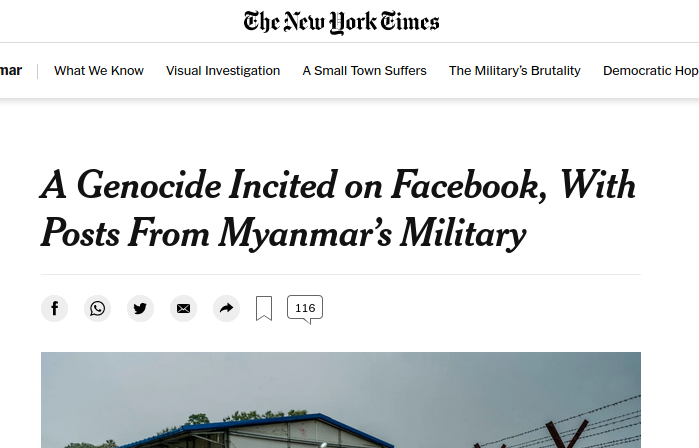
\includegraphics[width = \textwidth, height = .85\textheight, keepaspectratio]{figures/Myanmar.png}

\end{frame}

\note{It does not always need to be a financial motivation behind these social engineering attacks.

Propaganda is another form of social engineering. Crafting messages, memes, news stories to play into the same emotional mechanisms of hope, fear, urgency, in-group, out-group dynamics.

Social media allows these propaganda efforts from both domestic and foreign sources to propagate like they never did before.}

\begin{frame}
    \frametitle{Not Just a Third World Problem}
    
    \centering

    \movie{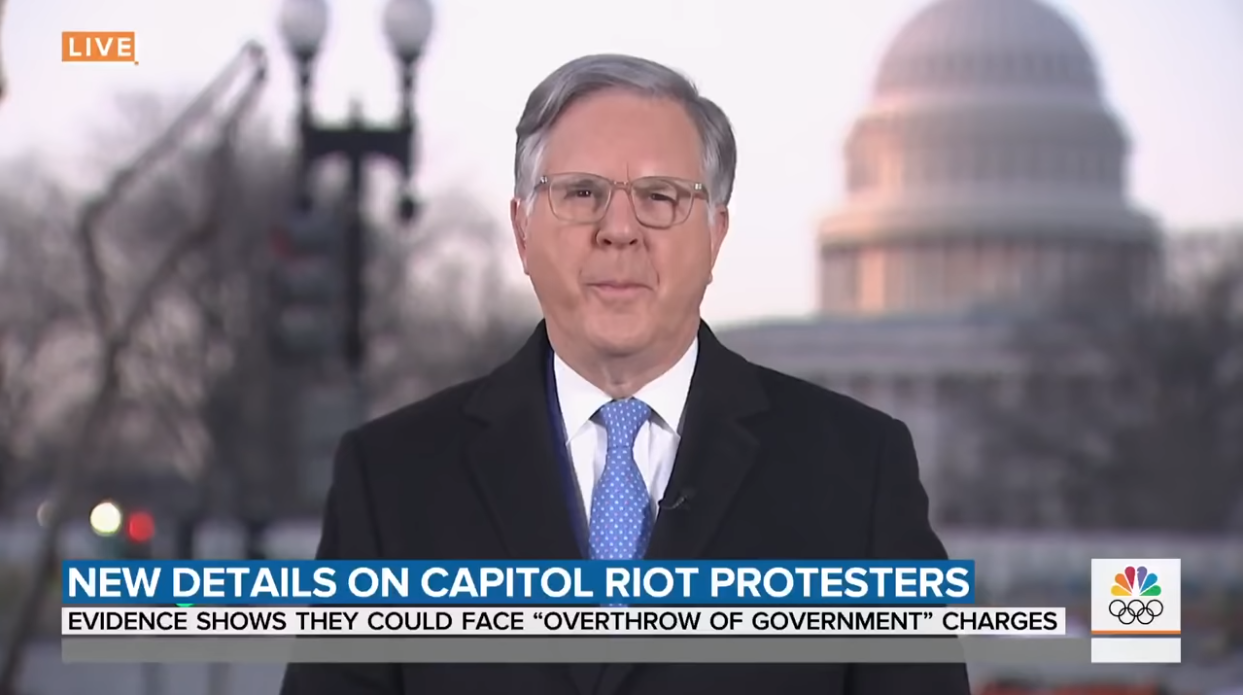
\includegraphics[width = \textwidth]{figures/Riot.png}}{figures/Riot.mp4}

\end{frame}

\note{When people think of propaganda, they often think of Nazi Germany, Soviet Russia, or China.

Unfortunately, Western democracies are also subject to a lot of propaganda. Maybe even more so as the citizens' opinions actually matter.}

\begin{frame}
	\frametitle{How Did It Get So Bad}
    \centering
	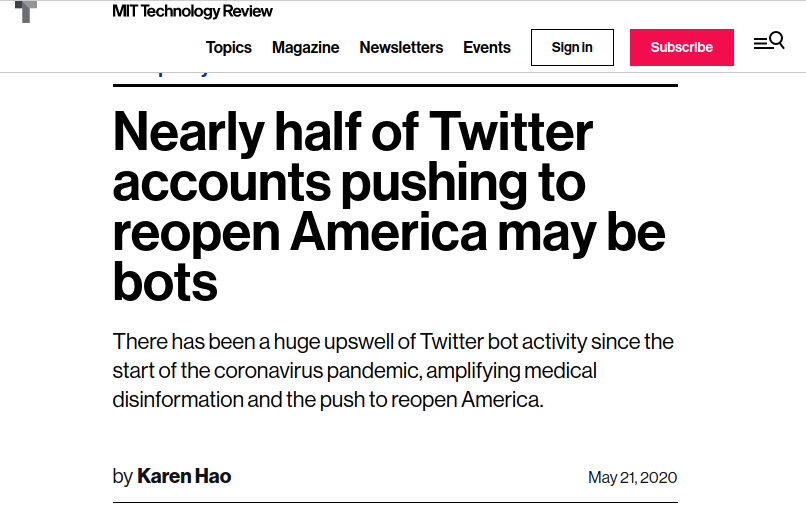
\includegraphics[width = \textwidth, height = .85\textheight, keepaspectratio]{figures/Bots.png}

\end{frame}

\note{Whether it be political or financial, these manipulation operations are profitable.

The forces behind them are no longer just some trolls looking for shits and giggles online.

They make money either through ads that are served, or through their handlers paying them for propaganda.

They fabricate these stories and then distribute them through social networks through sock puppet accounts and groups designed to amplify their message.

It is well known that various governments now operate ``Troll Farms'' where government employees, create and spread misinformation inside or outside their own countries.}


\begin{frame}
    \frametitle{What Can Be Done}
    
    Ignore the false sense of urgency \vspace{1em}

    Acknowledge the emotions triggered \vspace{1em}

    Think rationally \vspace{1em}

    Verify and validate through multiple channels

\end{frame}

\note{What is in common in all these cases, whether it be vishing, pishing, scam, or propaganda is the appeal to raw emotions and the abandonment of logic.

Be aware of the way messages are designed to elicit these emotions and control them.

Use logic and evidence to verify validity of the claims.

Often these claims will pass a surface check, so you may need to dig deeper and use authoritative sources that are harder to manipulate.}




\end{document}
